% Options for packages loaded elsewhere
\PassOptionsToPackage{unicode}{hyperref}
\PassOptionsToPackage{hyphens}{url}
%
\documentclass[
  11pt,
]{article}
\usepackage{amsmath,amssymb}
\usepackage{lmodern}
\usepackage{setspace}
\usepackage{ifxetex,ifluatex}
\ifnum 0\ifxetex 1\fi\ifluatex 1\fi=0 % if pdftex
  \usepackage[T1]{fontenc}
  \usepackage[utf8]{inputenc}
  \usepackage{textcomp} % provide euro and other symbols
\else % if luatex or xetex
  \usepackage{unicode-math}
  \defaultfontfeatures{Scale=MatchLowercase}
  \defaultfontfeatures[\rmfamily]{Ligatures=TeX,Scale=1}
\fi
% Use upquote if available, for straight quotes in verbatim environments
\IfFileExists{upquote.sty}{\usepackage{upquote}}{}
\IfFileExists{microtype.sty}{% use microtype if available
  \usepackage[]{microtype}
  \UseMicrotypeSet[protrusion]{basicmath} % disable protrusion for tt fonts
}{}
\usepackage{xcolor}
\IfFileExists{xurl.sty}{\usepackage{xurl}}{} % add URL line breaks if available
\IfFileExists{bookmark.sty}{\usepackage{bookmark}}{\usepackage{hyperref}}
\hypersetup{
  hidelinks,
  pdfcreator={LaTeX via pandoc}}
\urlstyle{same} % disable monospaced font for URLs
\usepackage[margin=1in]{geometry}
\usepackage{longtable,booktabs,array}
\usepackage{calc} % for calculating minipage widths
% Correct order of tables after \paragraph or \subparagraph
\usepackage{etoolbox}
\makeatletter
\patchcmd\longtable{\par}{\if@noskipsec\mbox{}\fi\par}{}{}
\makeatother
% Allow footnotes in longtable head/foot
\IfFileExists{footnotehyper.sty}{\usepackage{footnotehyper}}{\usepackage{footnote}}
\makesavenoteenv{longtable}
\usepackage{graphicx}
\makeatletter
\def\maxwidth{\ifdim\Gin@nat@width>\linewidth\linewidth\else\Gin@nat@width\fi}
\def\maxheight{\ifdim\Gin@nat@height>\textheight\textheight\else\Gin@nat@height\fi}
\makeatother
% Scale images if necessary, so that they will not overflow the page
% margins by default, and it is still possible to overwrite the defaults
% using explicit options in \includegraphics[width, height, ...]{}
\setkeys{Gin}{width=\maxwidth,height=\maxheight,keepaspectratio}
% Set default figure placement to htbp
\makeatletter
\def\fps@figure{htbp}
\makeatother
\setlength{\emergencystretch}{3em} % prevent overfull lines
\providecommand{\tightlist}{%
  \setlength{\itemsep}{0pt}\setlength{\parskip}{0pt}}
\setcounter{secnumdepth}{-\maxdimen} % remove section numbering
\ifluatex
  \usepackage{selnolig}  % disable illegal ligatures
\fi

\author{}
\date{\vspace{-2.5em}}

\begin{document}

\setstretch{1.25}
\hypertarget{anexos}{%
\section{Anexos}\label{anexos}}

\hypertarget{tabelas}{%
\subsection{Tabelas}\label{tabelas}}

~Tabela 3: Pontos de ocorrências de \emph{Encholirium subsecundum}
(Barker Mez).

\begin{longtable}[]{@{}
  >{\raggedright\arraybackslash}p{(\columnwidth - 8\tabcolsep) * \real{0.24}}
  >{\raggedright\arraybackslash}p{(\columnwidth - 8\tabcolsep) * \real{0.19}}
  >{\raggedright\arraybackslash}p{(\columnwidth - 8\tabcolsep) * \real{0.19}}
  >{\raggedright\arraybackslash}p{(\columnwidth - 8\tabcolsep) * \real{0.19}}
  >{\raggedright\arraybackslash}p{(\columnwidth - 8\tabcolsep) * \real{0.19}}@{}}
\toprule
Estado & Município & Longitude & Latitude & Referência \\
\midrule
\endhead
Minas Gerais & Belo Horizonte & -43.93780 & -19.92080 & Fundação
Zoo-Botânica de Belo Horizonte \\
Minas Gerais & Santana do Riacho & -43.71440 & -19.16890 & Fundação
Zoo-Botânica de Belo Horizonte \\
Minas Gerais & Conceição do Mato Dentro & -43.42500 & -19.03720 &
Fundação Zoo-Botânica de Belo Horizonte \\
Minas Gerais & Serro & -43.37940 & -18.60470 & Coleção da Escola
Superior de Agronomia Luiz de Queiroz - USP \\
Minas Gerais & Serro & -43.44500 & -18.47250 & Herbário do Museu
Nacional \\
Minas Gerais & Jequitaí & -44.44560 & -17.23560 & Coleção da
Universidade Federal de Viçosa \\
Minas Gerais & Buenópolis & -44.18000 & -17.87330 & Coleção da
Universidade Federal de Viçosa \\
Minas Gerais & Buenópolis & -44.23389 & -17.92389 & Coleção da
Universidade Federal do Maranhão \\
Minas Gerais & Buenópolis & -44.24944 & -17.90917 & Coleção da
Universidade Federal do Maranhão \\
Minas Gerais & Santana do Riacho & -43.71440 & -19.16890 & Coleção da
Universidade Federal de Viçosa \\
Minas Gerais & Mariana & -43.41610 & -20.37780 & Coleção da Universidade
Federal de Viçosa \\
Minas Gerais & Datas & -43.65580 & -18.44560 & Herbário do Museu
Botânico Municipal \\
Minas Gerais & Joaquim Felício & -44.17220 & -17.75750 & Coleção da
Universidade Estadual de Feira de Santana \\
Minas Gerais & Joaquim Felício & -44.29190 & -17.69890 & The New York
Botanical Garden \\
Minas Gerais & Joaquim Felício & -44.17220 & -17.75750 & Herbário da
Universidade Estadual de Feira de Santana \\
Minas Gerais & Santana do Riacho & -43.71440 & -19.16890 & Instituto de
Botânica \\
Minas Gerais & Penha da França & -43.83333 & -18.83333 & Coleção da
Universidade de Brasília \\
Minas Gerais & Montes Claros & -43.86170 & -16.73500 & Coleção da
UNICAMP \\
Minas Gerais & Santo Antônio do Itambé & -43.33944 & -18.45694 &
Herbário da UFMG \\
Minas Gerais & Pedro Leopoldo & -44.04310 & -19.61810 & Herbário da
UFMG \\
Minas Gerais & Itacambira & -43.30890 & -17.06470 & Herbário da UFMG \\
Minas Gerais & Dom Joaquim & -43.23333 & -18.86667 & Herbário do Museu
do Jardim Botânico do Rio de Janeiro \\
Minas Gerais & Mato Verde & -42.77889 & -15.38667 & Herbário do Museu do
Jardim Botânico do Rio de Janeiro \\
Minas Gerais & Santana de Pirapama & -43.75556 & -19.00611 & Herbário do
Museu do Jardim Botânico do Rio de Janeiro \\
Minas Gerais & Diamantina & -43.55278 & -18.35500 & Herbário do Museu do
Jardim Botânico do Rio de Janeiro \\
Minas Gerais & Diamantina & -43.62806 & -18.19194 & Herbário do Museu do
Jardim Botânico do Rio de Janeiro \\
Minas Gerais & Presidente Kubitschek & -43.55722 & -18.65389 &
@mariana2014 \\
Minas Gerais & Santana do Riacho & -43.51667 & 19.25000 & Herbário da
UFMG \\
Bahia & Itatim & -39.69810 & -12.71190 & Instituto de Botânica \\
Minas Gerais & Jaboticatubas & -43.74500 & -19.51360 & The New York
Botanical Garden \\
Minas Gerais & Jaboticatubas & -43.58333 & -19.16667 & Herbário do Museu
Nacional \\
\bottomrule
\end{longtable}

\clearpage

Tabela 4: Pontos de ocorrências de \emph{Lonchophylla bokermanni}
(Sazima, Vizotto \& Taddei).

\begin{longtable}[]{@{}
  >{\raggedright\arraybackslash}p{(\columnwidth - 8\tabcolsep) * \real{0.22}}
  >{\raggedright\arraybackslash}p{(\columnwidth - 8\tabcolsep) * \real{0.25}}
  >{\raggedright\arraybackslash}p{(\columnwidth - 8\tabcolsep) * \real{0.18}}
  >{\raggedright\arraybackslash}p{(\columnwidth - 8\tabcolsep) * \real{0.18}}
  >{\raggedright\arraybackslash}p{(\columnwidth - 8\tabcolsep) * \real{0.17}}@{}}
\toprule
Estado & Município & Longitude & Latitude & Referência \\
\midrule
\endhead
Minas gerais & Jaboticatubas & -43.74472 & -19.51361 & Coleção de
Mamíferos do Museu de Zoologia da UNICAMP \\
Minas gerais & Jaboticatubas & -43.60000 & -19.270000 &
@nascimento2013 \\
Minas gerais & Serra do Cipó & -43.60000 & -19.26667 & Coleção de
Mamíferos do Museu de Zoologia da UNICAMP \\
Minas gerais & Itambé do Mato Dentro & -43.349444 & -19.410278 &
@nascimento2013 \\
Minas gerais & Diamantina & -43.516667 & -18.383333 & @dias2013 \\
Minas gerais & Diamantina & -43.383333 & -18.383333 & @almeida2016 \\
Bahia & Caetité & -42.500000 & -14.266667 & @claudio2018 \\
Bahia & Ourolândia & -41.083333 & -11.083333 & @claudio2018 \\
\bottomrule
\end{longtable}

\clearpage

Tabela 5: Descrição das variáveis bioclimáticas derivadas de valores de
temperatura e pluviosidade {[}@worldclim{]}.

\begin{longtable}[]{@{}cc@{}}
\toprule
Variáveis bioclimáticas & Descrição \\
\midrule
\endhead
Bio 1 & Temperatura média anual \\
Bio 2 & Intervalo médio diurno (Média mensal (máx. temp. - mín
temp.)) \\
Bio 3 & Isotermalidade \\
Bio 4 & Sazonalidade de Temperatura (desvio padrão *100) \\
Bio 5 & Temperatura máxima do mês mais quente \\
Bio 6 & Temperatura mínima do mês mais frio \\
Bio 7 & Intervalo da temperatura anual \\
Bio 8 & Média da temperatura do quarto de ano mais úmido \\
Bio 9 & Média da temperatura do quarto de ano mais seco \\
Bio 10 & Média da temperatura do quarto de ano mais quente \\
Bio 11 & Média da temperatura do quarto de ano mais frio \\
Bio 12 & Precipitação anual \\
Bio 13 & Precipitação do mês mais frio \\
Bio 14 & Precipitação do mês mais seco \\
Bio 15 & Sazonalidade de precipitação (Coeficiente de variação) \\
Bio 16 & Precipitação do quadrimestre mais úmido \\
Bio 17 & Precipitação do quadrimestre mais seco \\
Bio 18 & Precipitação do quadrimestre mais quente \\
Bio 19 & Precipitação do quadrimestre mais frio \\
\bottomrule
\end{longtable}

\clearpage

Tabela 6: Valores VIF das variáveis sem problema de colinearidade (VIF
\textless{} 10) da espécie \emph{E. subsecundum}.

\begin{longtable}[]{@{}ll@{}}
\toprule
Variável & VIF \\
\midrule
\endhead
Bio 3 & 4.266921 \\
Bio 4 & 6.135108 \\
Bio 7 & 7.469114 \\
Bio 9 & 2.401162 \\
Bio 13 & 6.836922 \\
Bio 14 & 6.308869 \\
Bio 19 & 4.786559 \\
\bottomrule
\end{longtable}

Tabela 7: Valores VIF das variáveis sem problema de colinearidade (VIF
\textless{} 10) da espécie \emph{L. bokermanni}.

\begin{longtable}[]{@{}ll@{}}
\toprule
Variável & VIF \\
\midrule
\endhead
Bio 15 & 1.200694 \\
Bio 18 & 1.200694 \\
\bottomrule
\end{longtable}

\clearpage

Tabela 8: Contração, expansão ou não alteração relativa (em porcentagem)
para a espécie de planta e morcego sob os dois cenários climáticos
futuro, com relação à distribuição presente.

\begin{longtable}[]{@{}
  >{\raggedright\arraybackslash}p{(\columnwidth - 8\tabcolsep) * \real{0.31}}
  >{\raggedright\arraybackslash}p{(\columnwidth - 8\tabcolsep) * \real{0.19}}
  >{\raggedright\arraybackslash}p{(\columnwidth - 8\tabcolsep) * \real{0.13}}
  >{\raggedright\arraybackslash}p{(\columnwidth - 8\tabcolsep) * \real{0.13}}
  >{\raggedright\arraybackslash}p{(\columnwidth - 8\tabcolsep) * \real{0.22}}@{}}
\toprule
Espécie & Cenário & Ganho (\%) & Perda (\%) & Sem alteração (\%) \\
\midrule
\endhead
\emph{Lonchophylla bokermanni} & RCP 4.5 (2050) & 0.67 & 37.65 &
61.68 \\
& RCP 8.5 (2050) & 0.06 & 58.12 & 41.81 \\
\emph{Encholirium subsecundum} & RCP 4.5 (2050) & 0.08 & 72.78 &
27.14 \\
& RCP 8.5 (2050) & 0.00 & 81.11 & 18.89 \\
\bottomrule
\end{longtable}

Tabela 9: Distribuição sem sobreposição (desencontro geográfico) entre
planta e morcego nos três cenários climáticos.

\begin{longtable}[]{@{}
  >{\raggedright\arraybackslash}p{(\columnwidth - 6\tabcolsep) * \real{0.20}}
  >{\raggedright\arraybackslash}p{(\columnwidth - 6\tabcolsep) * \real{0.12}}
  >{\raggedright\arraybackslash}p{(\columnwidth - 6\tabcolsep) * \real{0.23}}
  >{\raggedright\arraybackslash}p{(\columnwidth - 6\tabcolsep) * \real{0.45}}@{}}
\toprule
Espécie & Cenário & Área de desencontro geográfico & Porcentagem com
relação à distribuição da espécie no cenário \\
\midrule
\endhead
\emph{Lonchophylla bokermanni} & Presente & 130263.7 & 26.07 \\
& RCP 4.5 (2050) & 190714.7 & 61.56 \\
& RCP 8.5 (2050) & 127101.0 & 63.07 \\
\emph{Encholirium subsecundum} & Presente & 144095.6 & 28.06 \\
& RCP 4.5 (2050) & 21127.3 & 15.07 \\
& RCP 8.5 (2050) & 22603.2 & 23.30 \\
\bottomrule
\end{longtable}

\clearpage

\hypertarget{figuras}{%
\subsection{Figuras}\label{figuras}}

\begin{figure}

{\centering 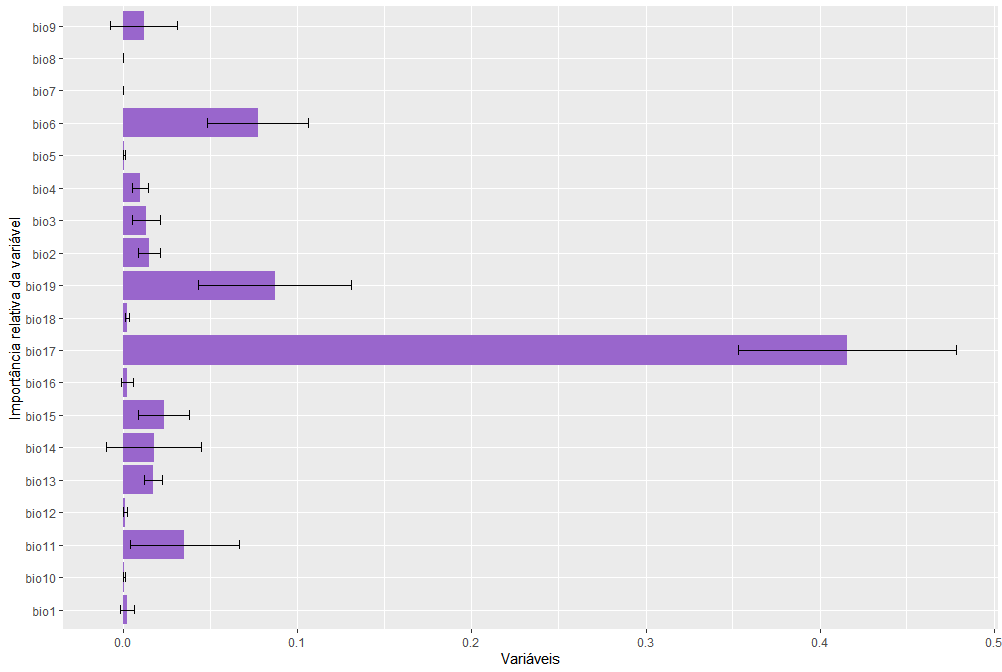
\includegraphics[width=0.73\linewidth]{../Rmarkdown/importancia_vars_planta} 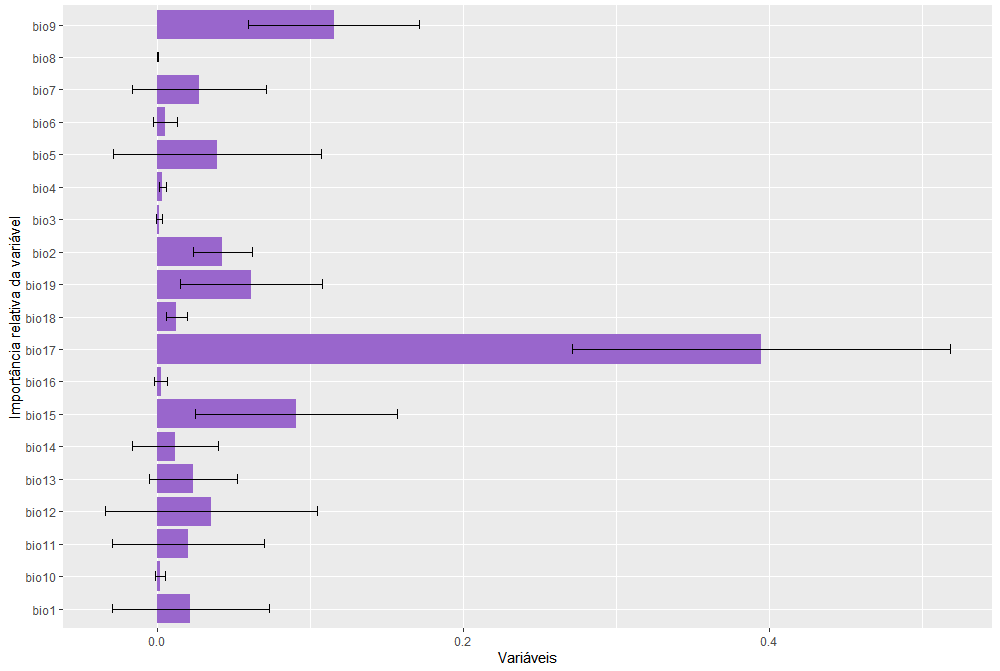
\includegraphics[width=0.73\linewidth]{importancia_vars_morcego} 

}

\caption{Importância relativa das variáveis para o modelo cheio da espécie de planta (acima) e para o morcego (abaixo).}\label{fig:vif}
\end{figure}

\clearpage

\begin{figure}

{\centering 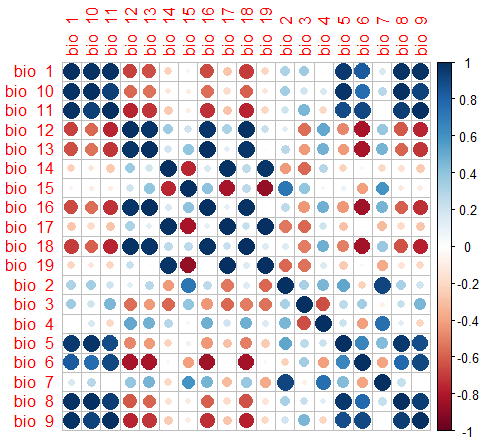
\includegraphics[width=0.49\linewidth]{../Dados/Resultados_VIF/E_subsecundum/Corr_plot_19_biovars} 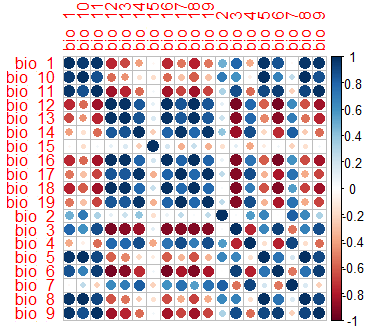
\includegraphics[width=0.49\linewidth]{../Dados/Resultados_VIF/L_bokermanni/Corr_plot_19_biovars} 

}

\caption{Matriz de correlação entre as variáveis bioclimáticas para a espécie E. subsecundum (à esquerda) e L. bokermanni (à direita)}\label{fig:VIF_subs}
\end{figure}

\begin{figure}
\centering
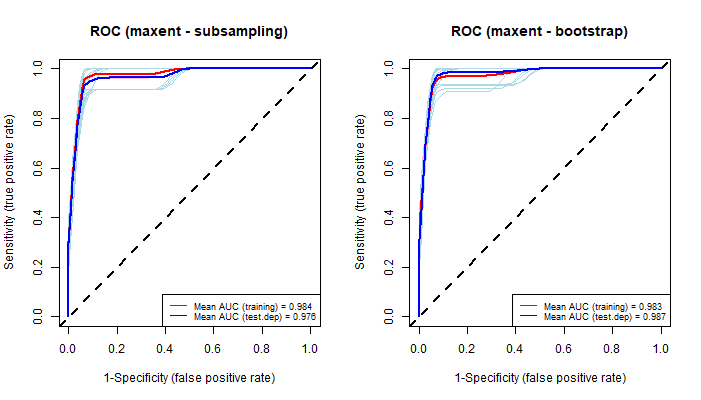
\includegraphics[width=0.8\textwidth,height=\textheight]{AUC_subsecundum.png}
\caption{Valores médios de AUC para os 25 modelos gerados da espécie
\emph{Encholirium subsecundum} com replicação por \emph{subsampling} (à
esquerda) e 25 por \emph{bootstrap} (à direita).}
\end{figure}

\begin{figure}
\centering
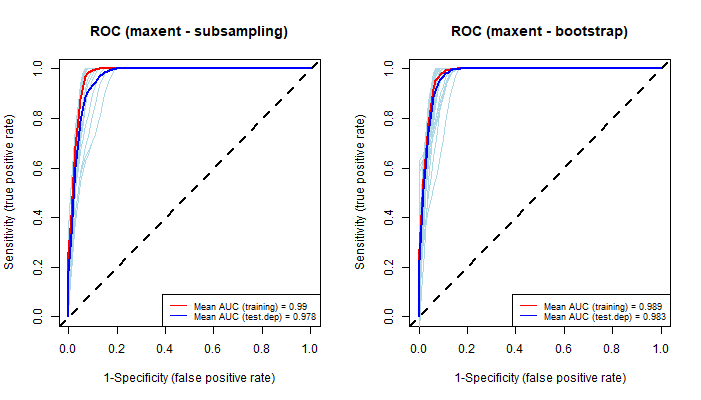
\includegraphics[width=0.8\textwidth,height=\textheight]{AUC_bokermanni.png}
\caption{Valores médios de AUC para os 25 modelos gerados da espécie
\emph{Lonchophylla bokermanni} com replicação por \emph{subsampling} (à
esquerda) e 25 por \emph{bootstrap} (à direita).}
\end{figure}

\begin{figure}
\centering
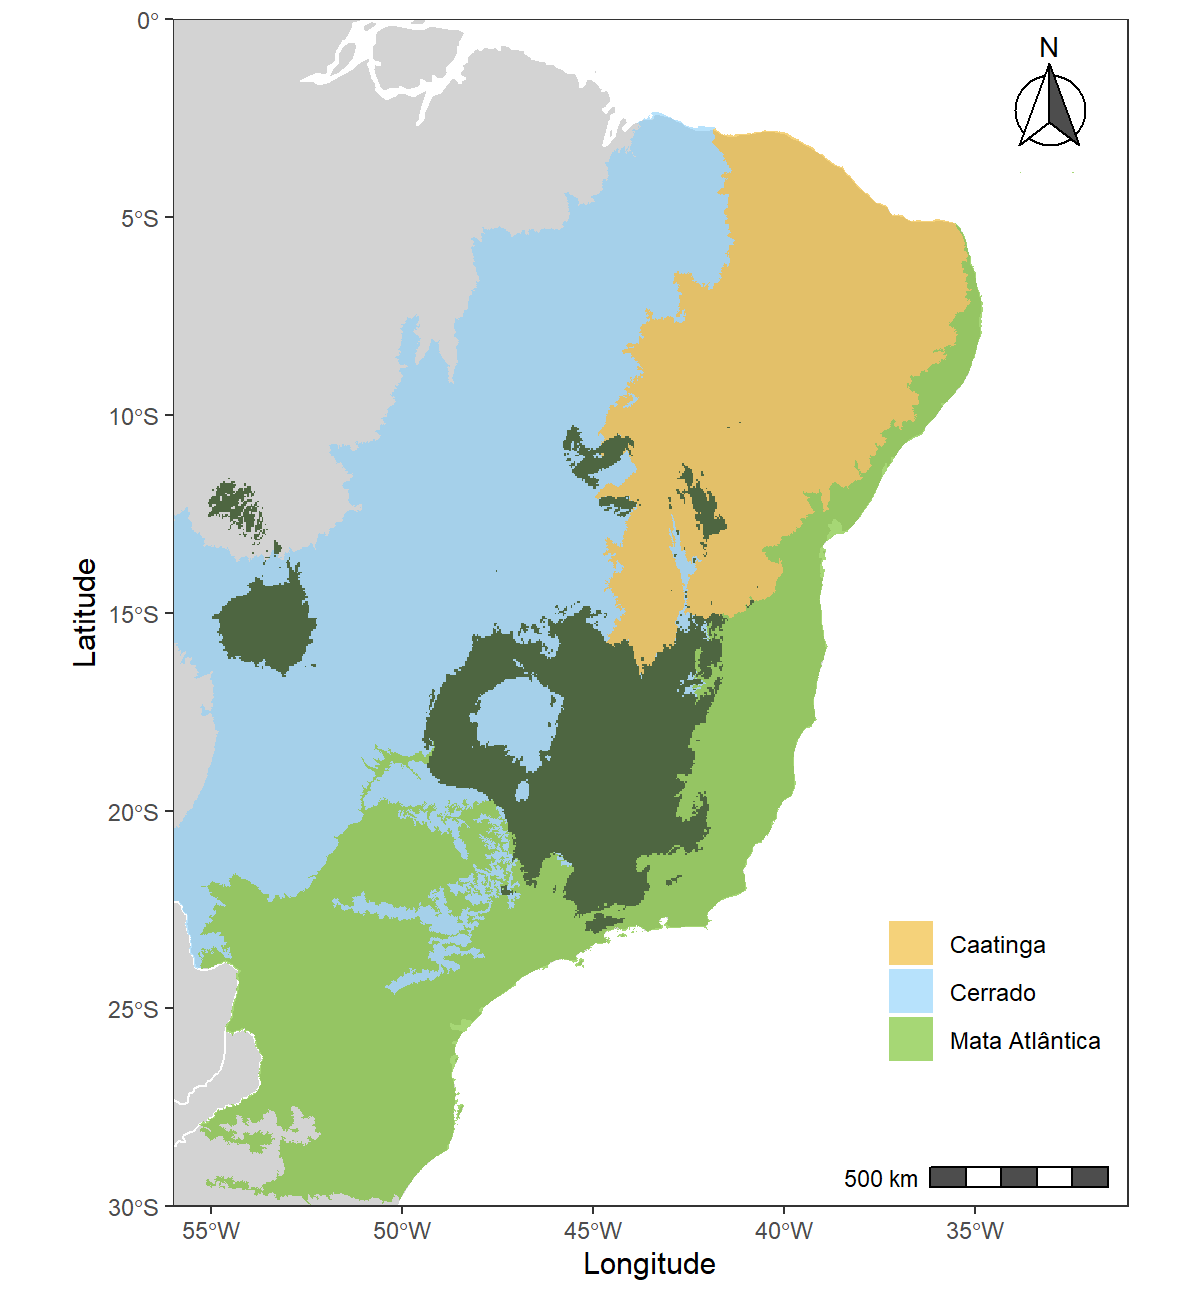
\includegraphics[width=1\textwidth,height=\textheight]{../Graficos/E_subsecundum_mapas_feitos/presente_e_biomas.jpeg}
\caption{Distribuição potencial de \emph{Encholirium subsecundum} (em
vermelho) para o presente.}
\end{figure}

\begin{figure}
\centering
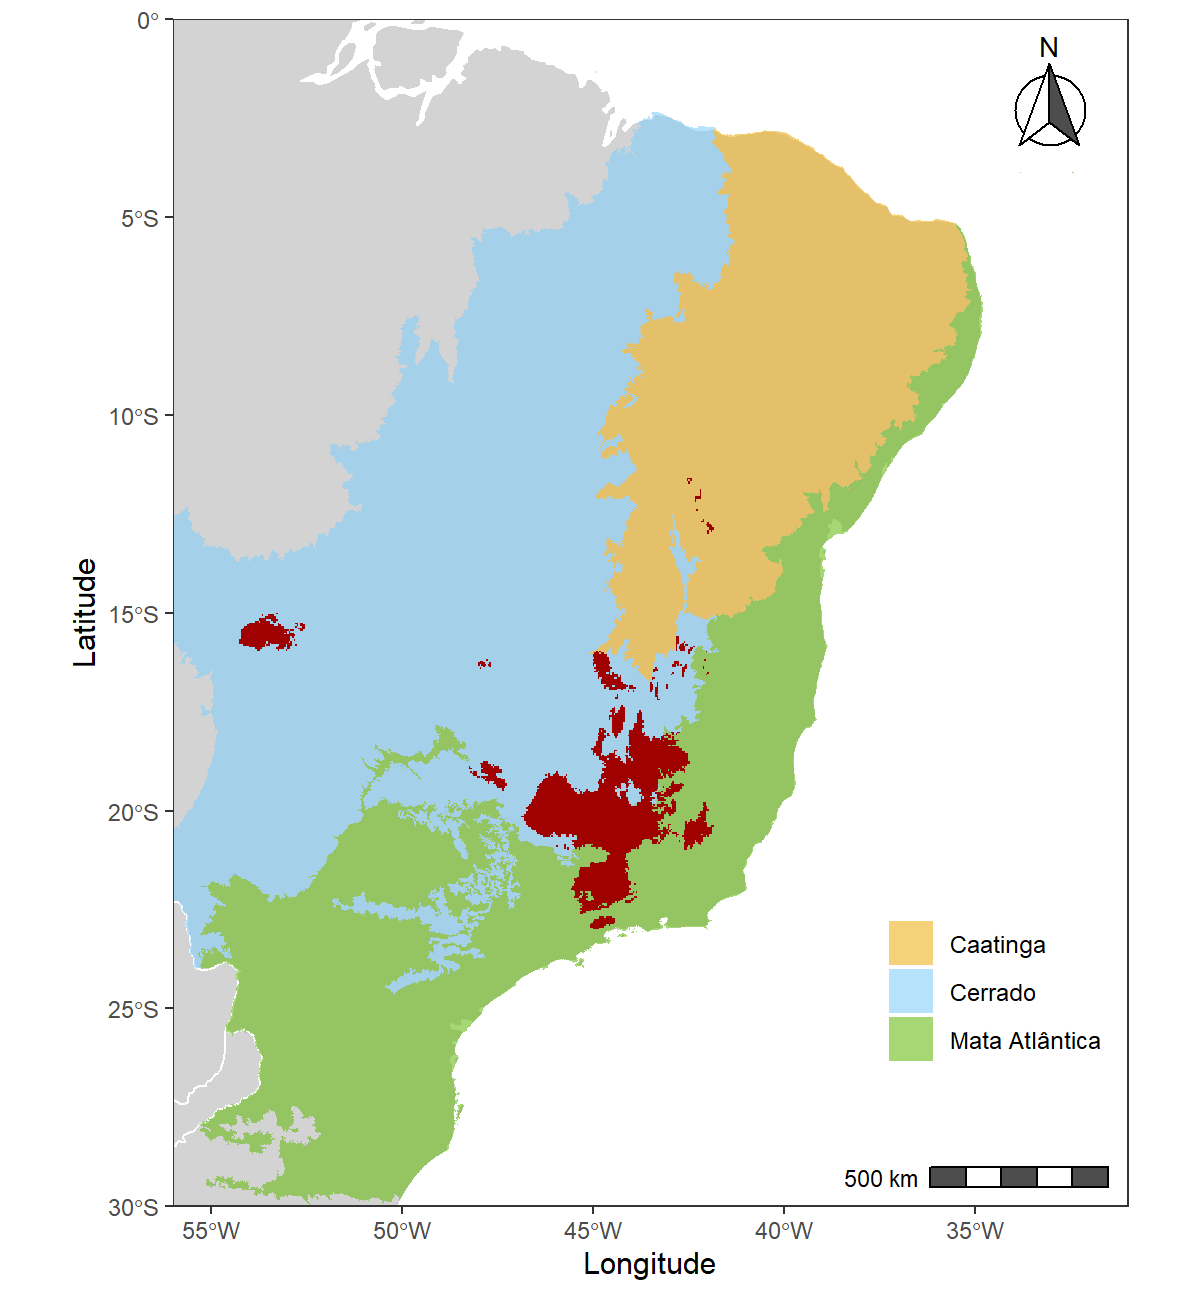
\includegraphics[width=1\textwidth,height=\textheight]{../Graficos/E_subsecundum_mapas_feitos/RCP45.jpeg}
\caption{Distribuição potencial de \emph{Encholirium subsecundum} (em
vermelho) para o cenário futuro de RCP 4.5 (2050).}
\end{figure}

\begin{figure}
\centering
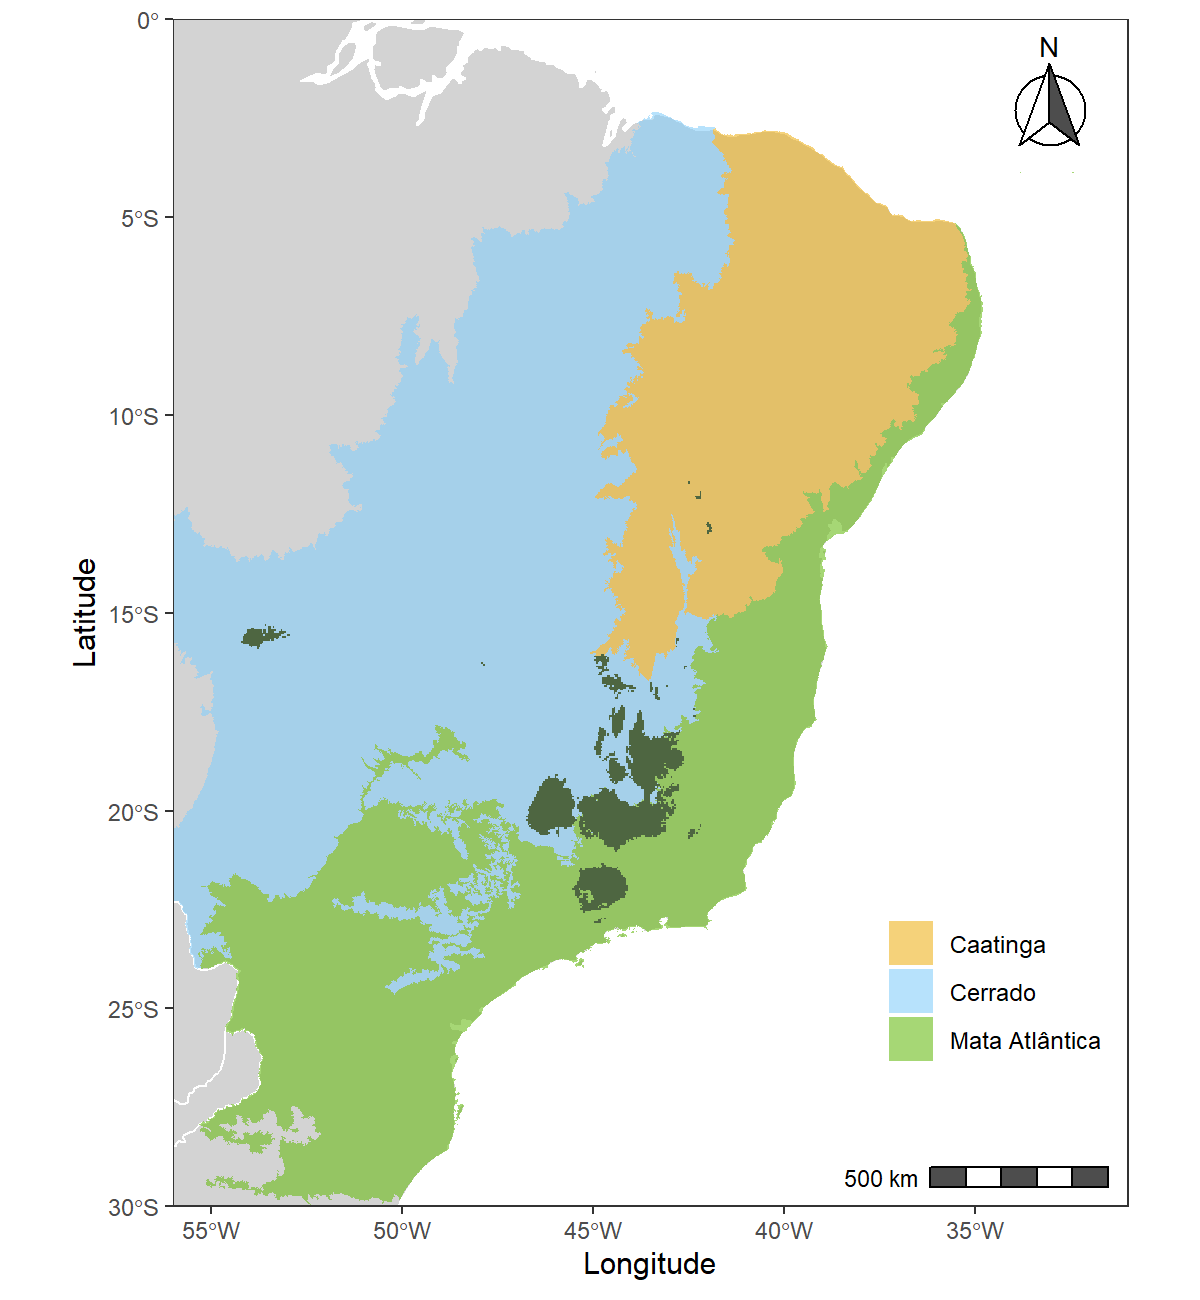
\includegraphics[width=1\textwidth,height=\textheight]{../Graficos/E_subsecundum_mapas_feitos/RCP85.jpeg}
\caption{Distribuição potencial de \emph{Encholirium subsecundum} (em
vermelho) para o cenário futuro de RCP 8.5 (2050).}
\end{figure}

\begin{figure}
\centering
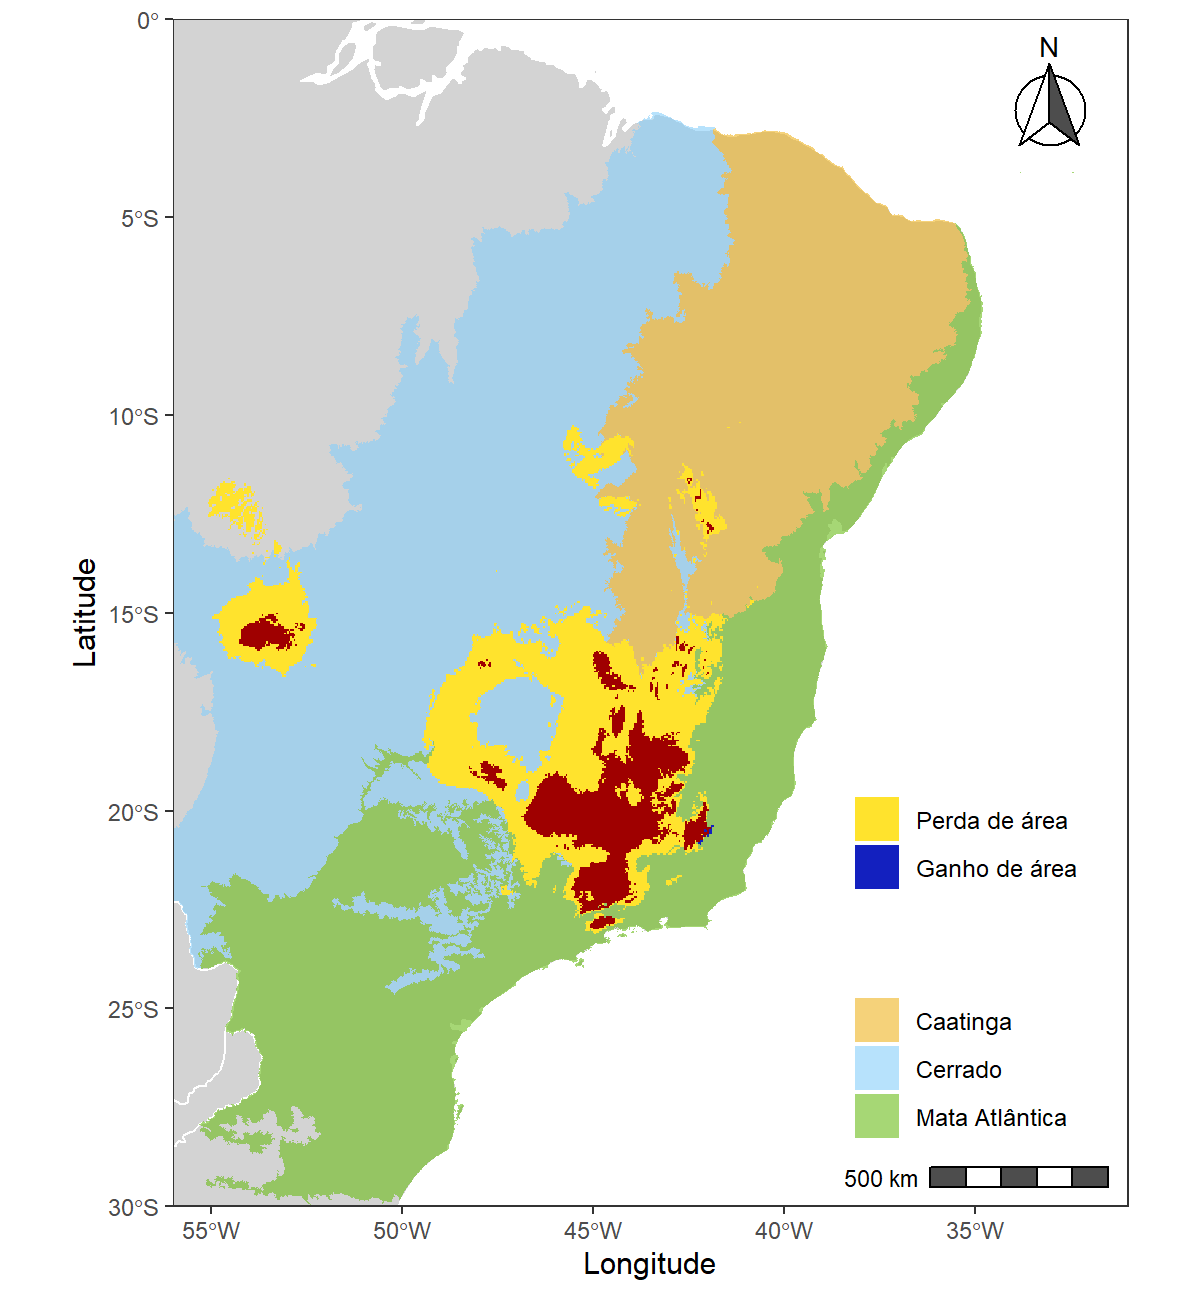
\includegraphics[width=1\textwidth,height=\textheight]{../Graficos/E_subsecundum_mapas_feitos/alteracao_RCP45.jpeg}
\caption{Mapa de alteração da distribuição potencial de
\emph{Encholirium subsecundum} no cenário RCP 4.5 (2050) em relação à
distribuição do presente. A área em vermelho, amarelo e azul representam
a distribuição sem alteração, perdida e ganha, respectivamente.}
\end{figure}

\begin{figure}
\centering
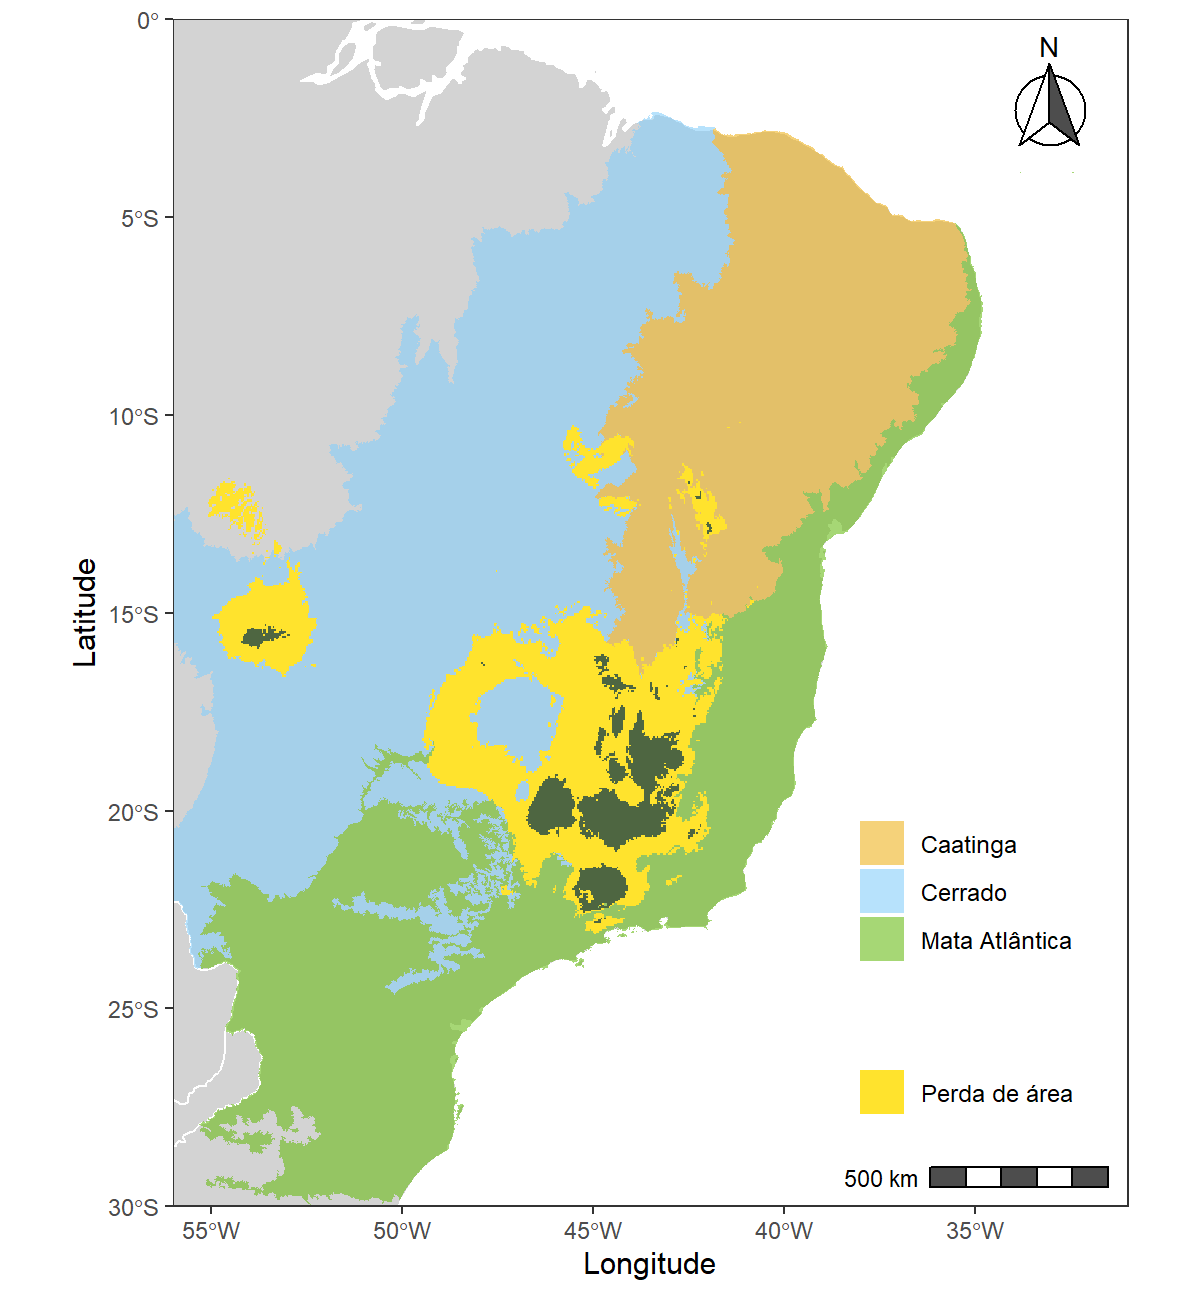
\includegraphics[width=1\textwidth,height=\textheight]{../Graficos/E_subsecundum_mapas_feitos/alteracao_RCP85.jpeg}
\caption{Mapa de alteração da distribuição potencial de
\emph{Encholirium subsecundum} no cenário RCP 8.5 (2050) em relação à
distribuição do presente. A área em vermelho e amarelo representam a
distribuição sem alteração e perdida. Não houve distribuição ganha da
planta no RCP 8.5.}
\end{figure}

\begin{figure}
\centering
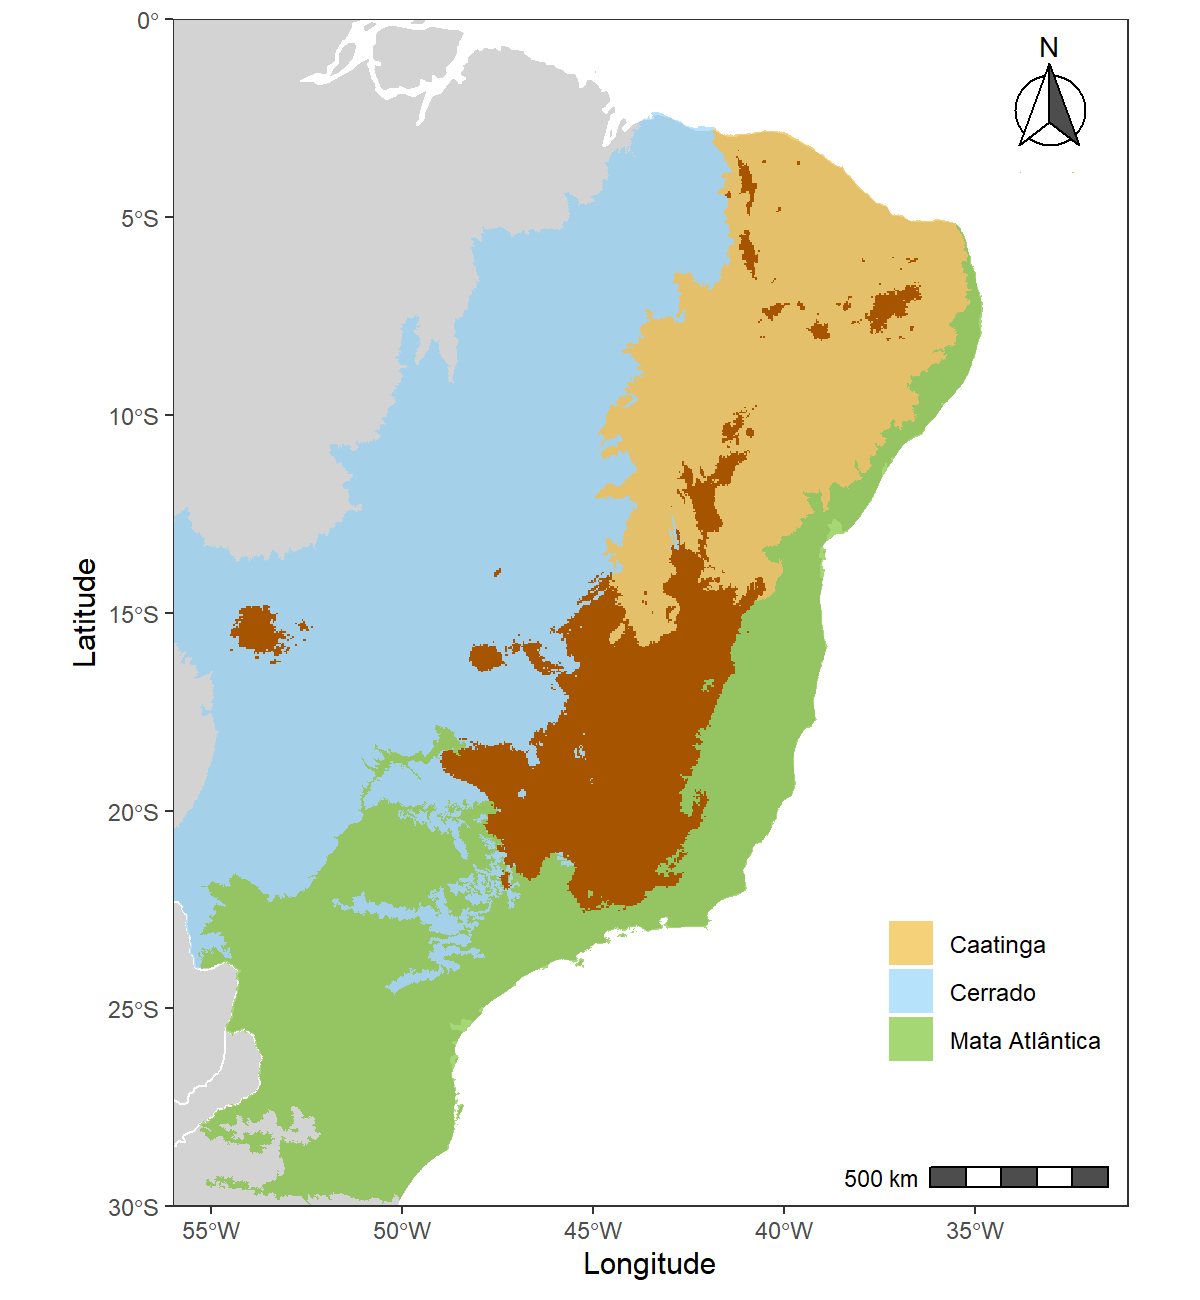
\includegraphics[width=1\textwidth,height=\textheight]{../Graficos/L_bokermanni_mapas_feitos/presente_e_biomas.jpeg}
\caption{Distribuição potencial de \emph{Lonchophylla bokermanni} (em
vermelho) para o presente.}
\end{figure}

\begin{figure}
\centering
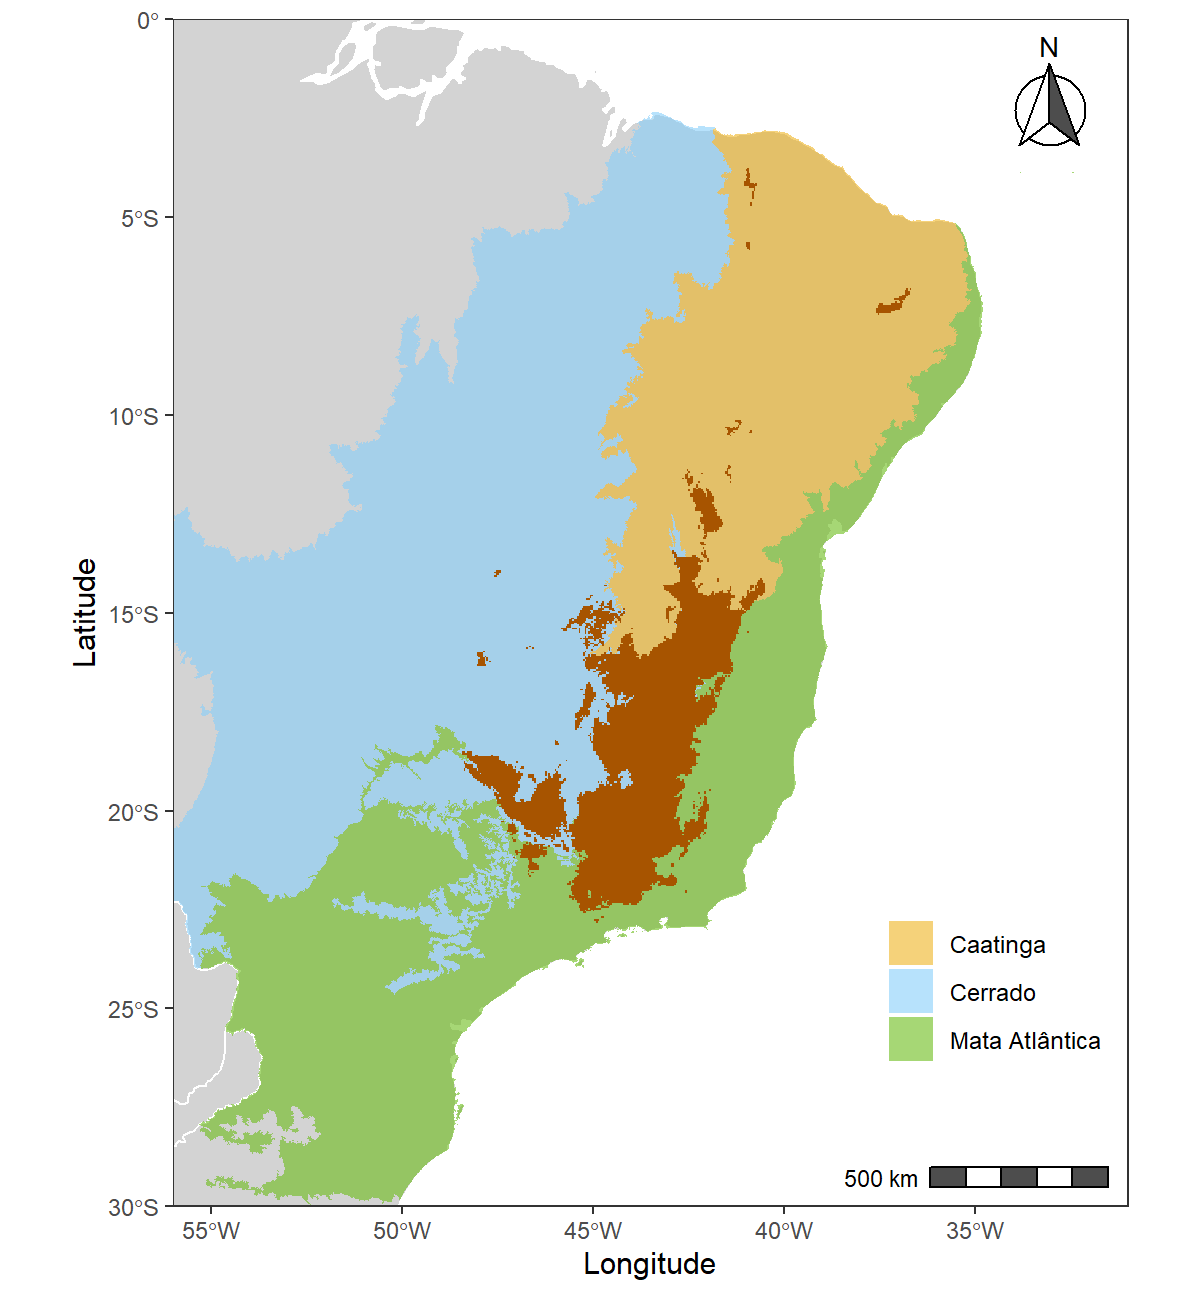
\includegraphics[width=1\textwidth,height=\textheight]{../Graficos/L_bokermanni_mapas_feitos/RCP45.jpeg}
\caption{Distribuição potencial de \emph{Lonchophylla bokermanni} (em
vermelho) para o cenário futuro de RCP 4.5.}
\end{figure}

\begin{figure}
\centering
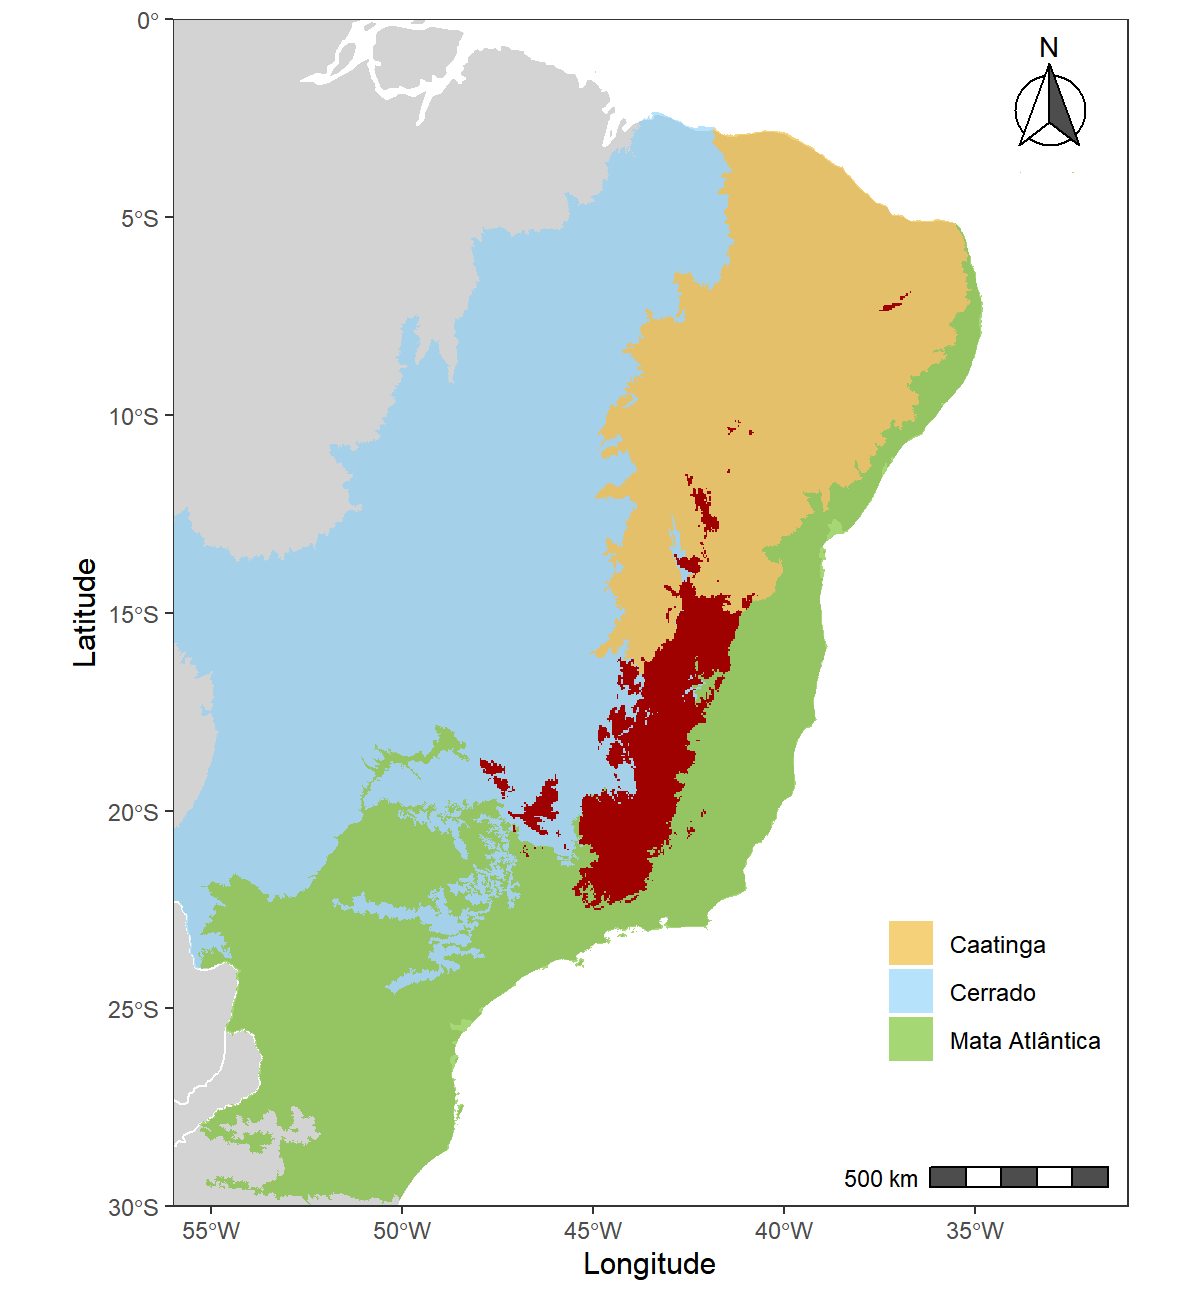
\includegraphics[width=1\textwidth,height=\textheight]{../Graficos/L_bokermanni_mapas_feitos/RCP85.jpeg}
\caption{Distribuição potencial de \emph{Lonchophylla bokermanni} (em
vermelho) para o cenário futuro de RCP 8.5.}
\end{figure}

\begin{figure}
\centering
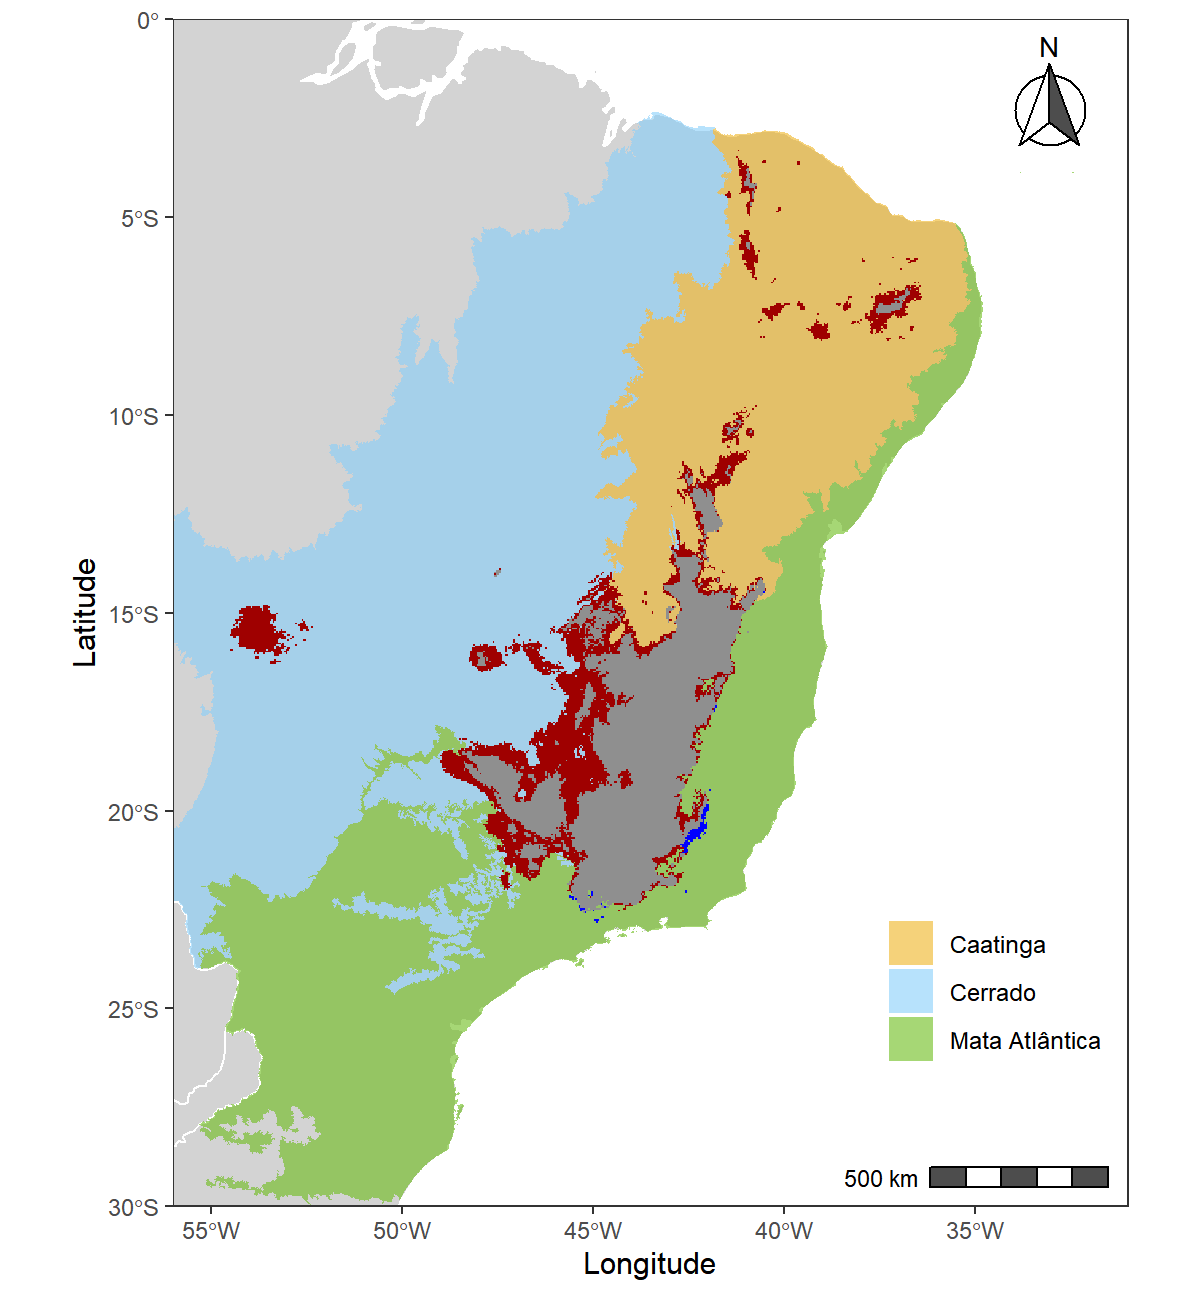
\includegraphics[width=1\textwidth,height=\textheight]{../Graficos/L_bokermanni_mapas_feitos/alteracao_RCP45.jpeg}
\caption{Mapa de alteração da distribuição potencial de
\emph{Lonchophylla bokermanni} no cenário RCP 4.5 (2050) em relação à
distribuição do presente. A área em vermelho, amarelo e azul representam
a distribuição sem alteração, perdida e ganha, respectivamente.}
\end{figure}

\begin{figure}
\centering
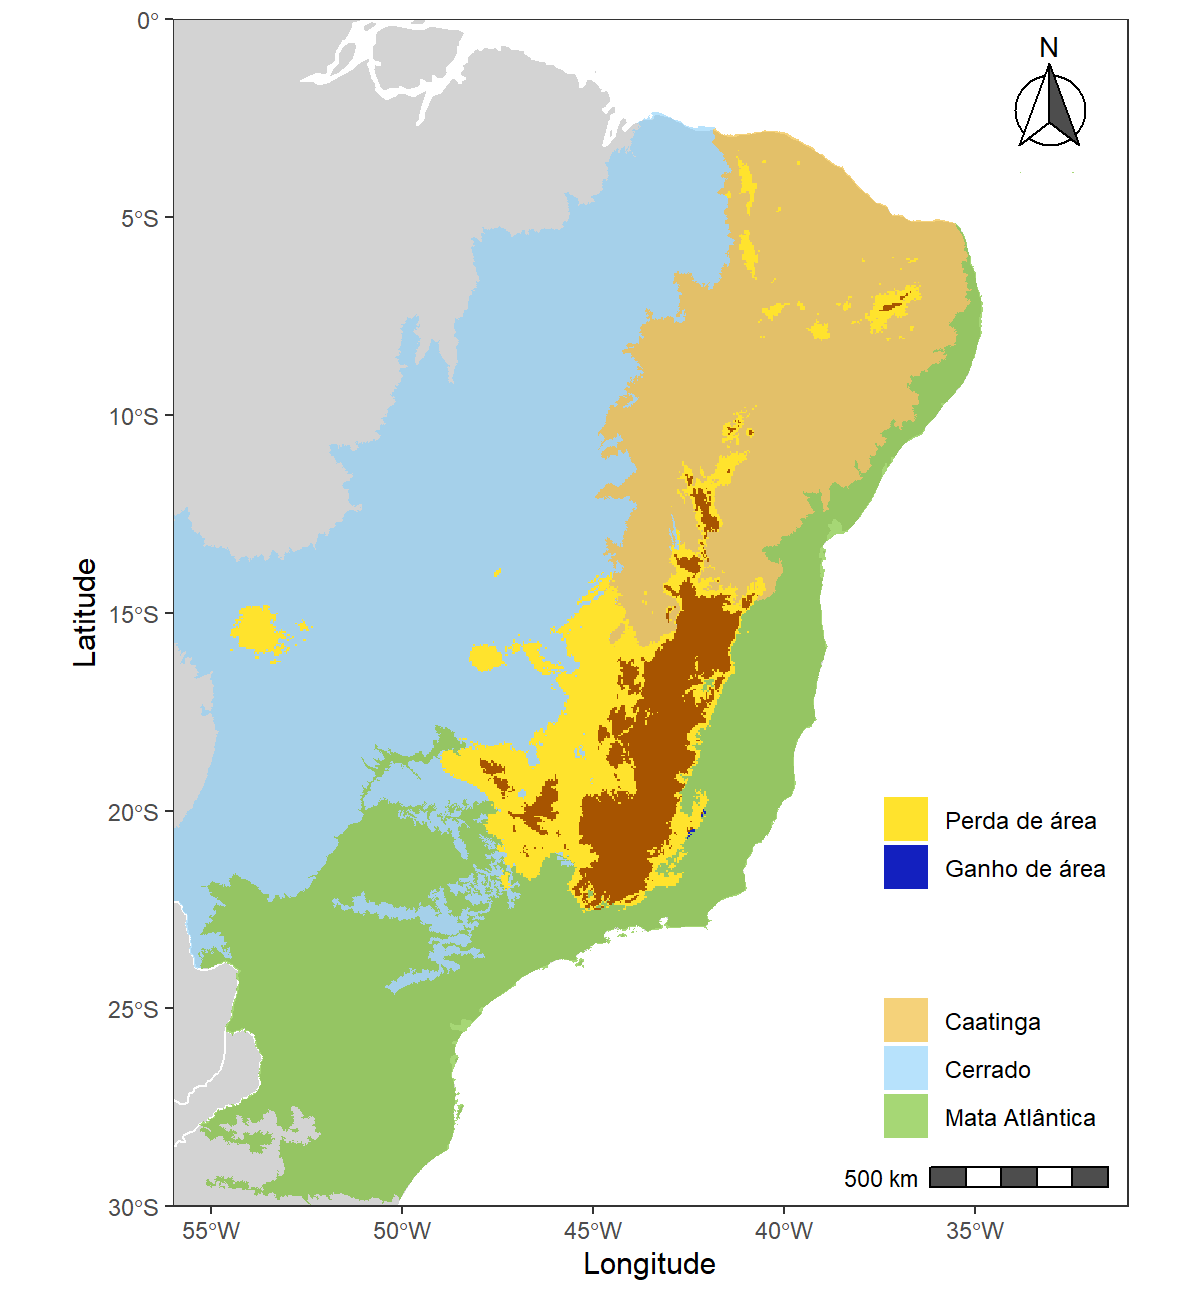
\includegraphics[width=1\textwidth,height=\textheight]{../Graficos/L_bokermanni_mapas_feitos/alteracao_RCP85.jpeg}
\caption{Mapa de alteração da distribuição potencial de
\emph{Lonchophylla bokermanni} no cenário RCP 8.5 (2050) em relação à
distribuição do presente. A área em vermelho, amarelo e azul representam
a distribuição sem alteração, perdida e ganha, respectivamente.}
\end{figure}

\end{document}
